\chapter{Methods} \label{chap:methods}

\cref{fig:1020EEG} shows a figure that we used with a caption. \cref{tab:interest} shows a table.


\begin{figure}[!htb]
	\centering
	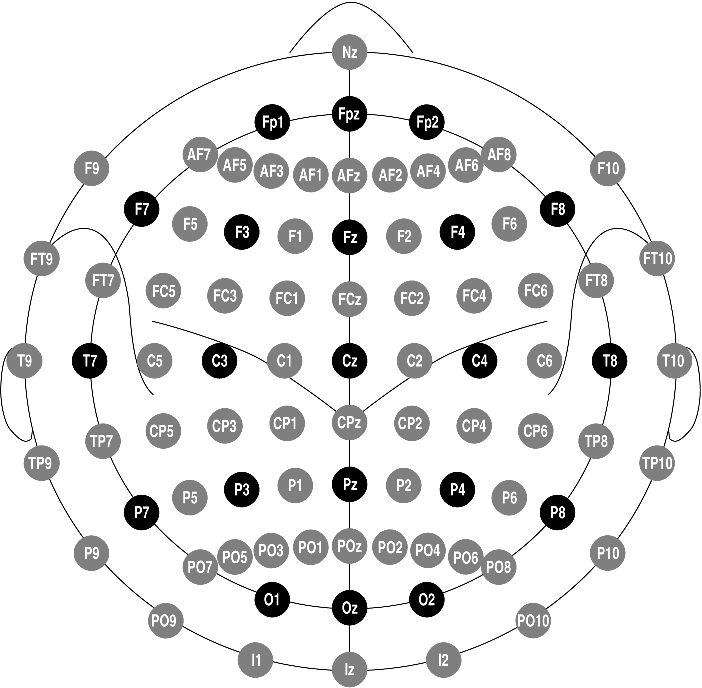
\includegraphics[width=2in]{figures/EEG_final_1020.pdf}
	\caption{An example of adding figures.}
	\label{fig:1020EEG}
\end{figure}

\begin{table}[!htb]
	\caption{A table of interest.}
	\label{tab:interest}
	\centering
	\begin{tabular}{cc}
		\toprule
		\textbf{Interest} & \textbf{Bank} \\
		\midrule
		1\% 	&	ASB bank \\
		2\% 	& 	ANZ bank \\
		3\%		& 	BNZ bank \\
		\bottomrule
	\end{tabular}
\end{table}